\documentclass{beamer}
\usepackage{siunitx,booktabs,xcolor,xspace,multirow,graphicx,lipsum}
\usepackage[spanish,mexico,es-noindentfirst]{babel}
\usepackage[utf8]{inputenc}
\usepackage{tikz}
\usepackage{tikzsymbols}
\usepackage{subcaption}
\usepackage{charter}
\usetheme{Madrid}
\usepackage{tcolorbox}
\usepackage{hyperref}
\usepackage{animate}
\usepackage{transparent}

\usepackage[T1]{fontenc}
\usepackage[export]{adjustbox}
\usetikzlibrary{positioning}
\usefonttheme{serif}
\DeclareUnicodeCharacter{2212}{\textendash}

\setbeamertemplate{frametitle}{
	\begin{beamercolorbox}[wd=\paperwidth, ht=0.85cm, sep=0.25cm]{frametitle}
		\begin{tikzpicture}[remember picture,overlay]
			\node[anchor=north east] at (current page.north east) {
\includegraphics[height=0.65cm]{fig/aries.png}};
		\end{tikzpicture}
		\usebeamerfont{frametitle}\bfseries\insertframetitle
	\end{beamercolorbox}
}
\definecolor{lightshadygreen}{RGB}{204, 230, 255}
\setbeamercovered{transparent}
\setbeamertemplate{caption}[numbered]
\setbeamercolor{frametitle}{bg=lightshadygreen,fg=black}
\setbeamercolor{author in head/foot}{bg=lightshadygreen,fg=blue}
\setbeamercolor{title in head/foot}{bg=lightshadygreen,fg=blue}
\setbeamercolor{date in head/foot}{bg=lightshadygreen,fg=blue}
\setbeamercolor{titlelike}{parent=structure,bg=lightshadygreen,fg=black}
\setbeamertemplate{section in toc}[sections numbered]
\setbeamertemplate{subsection in toc}[subsections numbered]
\setbeamerfont{section in toc}{series=\bfseries}
\setbeamercolor{section in toc}{fg=black}
\setbeamercolor{caption name}{fg=black}
\setbeamerfont{caption name}{series=\bfseries}
\setbeamerfont{caption}{size=\small}
\setbeamercolor{bibliography entry author}{fg=black}
\setbeamercolor{bibliography entry title}{fg=black} 
\setbeamertemplate{section in toc}{\inserttocsectionnumber.~\inserttocsection\par}
\setbeamertemplate{subsection in toc}{\hspace{1.5em}\inserttocsectionnumber.\inserttocsubsectionnumber~\inserttocsubsection\par}

% Apply the custom color to the frametitle
\setbeamercolor{frametitle}{bg=lightshadygreen, fg=black}

\title[\textbf{Astro-AI Meeting}]{\textbf{Generative AI for Image Reconstruction in Intensity Interferometry: a First Attempt}}
\author[\textbf{Km Nitu Rai}]{\textbf{\underline{Speaker:}} Km Nitu Rai \vspace{0.01cm} \\ 
	{\scriptsize \underline{\textcolor{blue}{niturai201296@gmail.com}}} \\
	{\scriptsize {\textbf{\underline{Contributers:}} Km Nitu Rai, Yuri van der Burg, Soumen Basak, Prasenjit Saha, and Subrata Sarangi}} \\
	{\scriptsize \underline{\textbf{\tiny Presenting at}}} \\	
	{\scriptsize \underline{\textcolor{blue}{Astro-AI Meeting at IUCAA Pune}}}}

\date{\vspace{-1cm}\textbf{24th April, 2024}}

\renewcommand{\maketitle}{
	\begin{figure}[!htb]
		\centering
		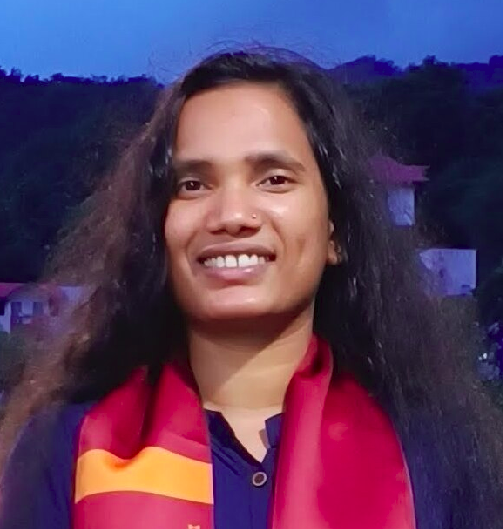
\includegraphics[height=2cm]{fig/team/Nitu.png}\hfill
		
\includegraphics[height=2cm]{fig/team/Yuri.png}\hfill
		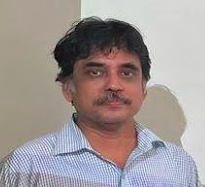
\includegraphics[height=2cm]{fig/team/Soumen.png}\hfill
		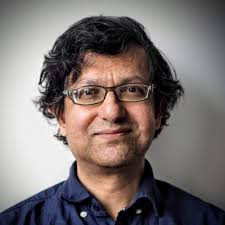
\includegraphics[height=2cm]{fig/team/Saha.jpeg}\hfill
		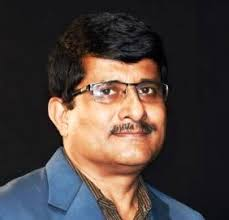
\includegraphics[height=2cm]{fig/team/Sarangi.jpeg}
	\end{figure}
	\vspace{-1cm}
	\titlepage
}




\definecolor{beamer_color}{RGB}{176,196,222} 
\begin{document}
	\maketitle

	\begin{frame}
		\centering  
		\visible<1-4>{
			\textbf{\textit{\textcolor{blue}{\underline{Objective}: High Resolution of Stellar Objects...}}}\\
			\vspace{0.4cm}
		}  
		\visible<2-4>{
			\textbf{\textit{\textcolor{red}{\underline{Limitation}: There Size of Aperture of Telescope...}}}\\
			\vspace{0.4cm}
		}
		
		\visible<3-4>{
			\textbf{\textit{\textcolor{blue}{\underline{Solution}: Interferometry Technique using Multiple Telescope...}}}\\
			\vspace{0.4cm}
		}
		
		\visible<4>{
			\textbf{\textit{\textcolor{red}{\underline{Challenges}: The Extraction of Lost Quantities for high resolution...}}}
		}
	\end{frame}

    \begin{frame}{Requirements of High Resolution}
    	\begin{columns}[c]
    		\column{0.6\textwidth}
    		\begin{itemize}
    			\item Stellar objects appear almost like point sources (milli-arcsecond or less).
    			\pause
    			\item Understanding stellar structure is crucial for stellar evolution.
    			\pause
    			\item High angular resolution is required to resolve stellar structure.
    			\pause
    			\item The Sun is the only star currently resolved in detail.
    		\end{itemize}
    		
    		\column{0.4\textwidth}
    		\begin{figure}
    			\centering
    			\vspace{-0.5cm}
    			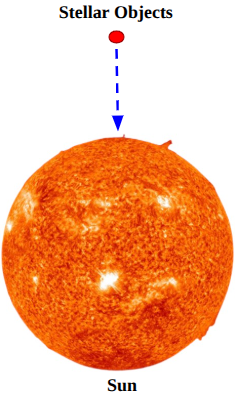
\includegraphics[width=0.85\textwidth]{fig/sun.png}
    		\end{figure}
    	\end{columns}
    \end{frame}

    \begin{frame}{Maximum Resolution with a Telescope}
    	\begin{columns}[c]
    		\column{0.6\textwidth}
    		\begin{itemize}
    			\item Resolution is limited by diffraction: $ \theta \sim \frac{\lambda}{D}$
    	    	\pause
    	    	\item Larger aperture $\Rightarrow$ better resolution
    	    	\pause
    	    	\item Gran Telescopio Canarias is limited to 13.3 milli-arcsecond scale on 550 nm.
    	    	\pause
    	    	\item For micro-arc-second resolution on 550 nm $\Rightarrow$ $D \approx 140 \, \rm km$.
    	    	\pause
    	    	\item There will be a limit on the size of the telescope: Handling problem.
    		\end{itemize}
    		
    		\column{0.4\textwidth}
    		\begin{figure}
    			\centering
    			\vspace{-0.5cm}
    			\includegraphics[width=0.75\textwidth]{fig/GTC_Resolve.png}
    		\end{figure}
    	\end{columns}
    \end{frame}
    
    \begin{frame}
    	\begin{figure}
    		\includegraphics[width=\textwidth]{fig/teles.png}
    	\end{figure}
    \end{frame}
    
    \begin{frame}{Interferometry: The Technique}
    	\begin{figure}
    		\centering
    		\vspace{-0.5cm}
    		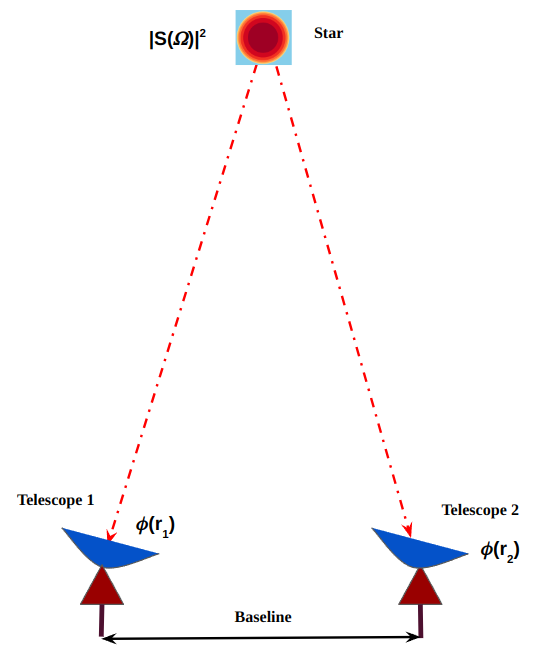
\includegraphics[width=0.4\linewidth]{fig/earth.png}
    	\end{figure}
    	\begin{itemize}
    		\item Two telescopes separated by a distance $B$ act like a single aperture.
    		\pause
    		\item Angular resolution: $\theta \sim \frac{\lambda}{B}$.
    		\pause
    		\item Interferometry measures correlation of signals from telescopes.
    	\end{itemize}
    \end{frame}

    \begin{frame}{The Measured Signal}
    \only<1-3>{
    	\begin{columns}[c]
    		\column{0.55\textwidth}
    		\begin{itemize}
    			\setlength{\itemsep}{5pt}
    			\item Photon flux from a star following black body radiation
    			\textcolor{blue}{\textbf{
    					\begin{equation*}
    						|S(\Omega)|^2 = \frac{{\nu^2}/{c^2}}{e^{{h\nu}/{kT(\Omega)}}-1}  
    						\label{eqn:fluxA} 
    			\end{equation*}}}
    			\visible<2->{
    				\item Fraunhofer diffraction for a light
    				\textcolor{blue}{\textbf{
    						\begin{equation*}
    							\phi(r, t) \propto \int e^{2\pi i(\nu/c) r.\Omega} e^{2\pi i(\nu/c) t} \, S(\Omega) \, d^2\Omega
    							\label{eqn:pi}
    			\end{equation*}}}}
    			\visible<3->{
    				\item The correlation in amplitudes
    				\textcolor{blue}{\textbf{
    						\begin{equation*}
    							\phi(r_1, t_1)\,\ast \, \phi^*(r_2, t_2) \propto \int e^{2\pi i (\nu/c)(r_1-r_2).\Omega} e^{2\pi i (\nu/c)(t_1-t_2).\Omega} \, |S(\Omega)|^2 \, d^2\Omega
    							\label{eqn:phi2}
    			\end{equation*}}}}
    		\end{itemize}
    		\column{0.45\textwidth}
    		\vspace{-1cm}
    		\visible<1-3>{
    			\only<1>{
    				\begin{center}
    					\includegraphics[width=0.95\linewidth]{../../ARIES/talk/fig/SI/star_1.png}
    			\end{center}}
    			\only<2>{
    				\begin{center}
    					\includegraphics[width=0.7\linewidth]{../../ARIES/talk/fig/SI/earth1.png}
    			\end{center}}
    			\only<3>{
    				\begin{center}
    					
\includegraphics[width=0.7\linewidth]{../../ARIES/talk/fig/SI/earth.png}
    		\end{center}}}
    \end{columns}}
    \end{frame}
    
\begin{frame}{The Measured Signal}
	\begin{itemize}\setlength{\itemsep}{6pt}
		\item Average over space and time provides first-order correlation
		\textcolor{blue}{\textbf{
				\begin{equation*}
					g^{(1)}(\mathbf{r}_1, t_1; \mathbf{r}_2, t_2) =
					\frac{\langle \phi^*(\mathbf{r}_1, t_1)\, \phi(\mathbf{r}_2, t_2) \rangle}
					{\sqrt{\langle |\phi(\mathbf{r}_1, t_1)|^2 \rangle \, \langle |\phi(\mathbf{r}_2, t_2)|^2 \rangle}}
		\end{equation*}}}
		\visible<2-4>{
		\item In interferometry: $g^{(1)} \rightarrow$ \textbf{complex visibility} $V(u,v)$}
		\visible<3-4>{
		\item It is also called Van Cittert Zernike theorem
		\[
		V(u,v) = \mathcal{F}\{|S(\Omega)|^2\}
		\]}
		\visible<4>{
		\item Signal measured in amplitude interferometry!!!}
	\end{itemize}
\end{frame}

\begin{frame}
	\centering
	\visible<1-2>{
		\textbf{\textit{\textcolor{blue}{\underline{Event Horizon Telescope (EHT)} - captured the first ever image of black hole using \underline{Radio Wavelength.}}}}
	}     
	\visible<2>{
		\centering
		\includegraphics[width=0.8\linewidth]{../../ARIES/talk/fig/EHT.png}
	}
\end{frame}

\begin{frame}
	\centering  
	\visible<1-2>{
		\textbf{\textit{\textcolor{blue}{What about \underline{Amplitude Interferometry on Optical Wavelength???}}}}\\
		\vspace{0.4cm}
	}  
	\visible<2>{
		\textbf{\textit{\textcolor{red}{For Better Resolution $\Rightarrow$ Longer Baseline}}}
	}
\end{frame}

\begin{frame}{The Limitation on Amplitude Interferometry}
	\begin{itemize}\setlength{\itemsep}{6pt}
		\item Requires \textbf{phase stability} at the level of wavelength ($\sim$ nm)
		\pause
		\item Optical path difference must be controlled with extreme precision
		\pause
		\item Atmospheric turbulence introduces rapid phase fluctuations
		\pause
		\item Sensitivity decreases for long baselines and faint sources
		\pause
		\item Practical baseline extension is limited (typically $\sim$ 100 m scale)
		\pause
		\item \textbf{Difficult to achieve very long baselines in optical range.}
	\end{itemize}
\end{frame}

\begin{frame}
	\centering
		\textbf{\textit{\textcolor{blue}{\underline{Let's talk} - \textcolor{red}{Hanbury Brown and Twiss (HBT) Interferometry} for \underline{High Resolution on Optical Range}....}}}
\end{frame}

\begin{frame}{}
	\centering
	\visible<1-2>{
		\textbf{\textit{\textcolor{blue}{Let's \underline{Have a Look} on Something OLD!!!}}}}\\
	\vspace{0.5cm}
	\visible<2>{
		\textbf{\textit{\textcolor{red}{A Brief Historical View of \underline{HBT Interferometry}, Unknown Before 1950s}}}}
\end{frame}

\begin{frame}{HBT Interferometry}
	\only<1-2>{
		\vspace{0.2cm}
		\visible<1-2>{
			\begin{figure}
				\includegraphics[width=0.8\linewidth]{../../ARIES/talk/fig/SI/int.png}
		\end{figure}}
		\vspace{-0.2cm}
		\begin{itemize}\setlength{\itemsep}{5pt}
			\visible<1->{
				\item What if there is correlation between intensity instead of amplitude.}
			\visible<2->{
				\item Robert \textbf{\textcolor{red}{Hanbury Brown and Twiss (HBT)}} lead this idea!!!}
	\end{itemize}}
	\only<3-6>{\vspace{-0.1cm}
		\visible<6>{
			\centering
			\begin{figure}
				\includegraphics[width=0.85\linewidth]{../../ARIES/talk/fig/hanbury.png}
		\end{figure}}
		\begin{itemize}\setlength{\itemsep}{5pt}
			\setlength\itemsep{0.5em}
			\visible<3-6>{
				\item Light was viewed as \textbf{\textcolor{red}{collection of individual photons}.}}
			\visible<4-6>{
				\item The \textcolor{blue}{\textbf{correlation of photons}} were detected from two places.}
			\visible<5-6>{
				\item Glauber, E. Wolf, and Leonard Mandel played an important role.}
			\visible<6>{
				\item \textcolor{blue}{\textbf{First Intensity Interferometer}} at Narrabri was installed in 1963.}
		\end{itemize}    
	}			
\end{frame}

\begin{frame}
	\begin{figure}
		\includegraphics[width=\textwidth]{fig/CTA.png}
	\end{figure}
\end{frame}

    \begin{frame}{The Intensity Interferometry}
    	\begin{itemize}\setlength{\itemsep}{-5pt}
    		\item Correlation also exist in Intensity (HBT Effect)
    		\textcolor{blue}{\textbf{\begin{equation*}
    					g^{(2)}(\mathbf{r}_1, t_1; \mathbf{r}_2, t_2) =
    					\frac{\langle I(\mathbf{r}_1, t_1) \, I(\mathbf{r}_2, t_2) \rangle}
    					{\langle I(\mathbf{r}_1, t_1) \rangle \, \langle I(\mathbf{r}_2, t_2) \rangle}
    					=
    					\frac{\langle |E(\mathbf{r}_1, t_1)|^2 \, |E(\mathbf{r}_2, t_2)|^2 \rangle}
    					{\langle |E(\mathbf{r}_1, t_1)|^2 \rangle \, \langle |E(\mathbf{r}_2, t_2)|^2 \rangle}    			
    		\end{equation*}}}
    	    \pause
    		\item Generalized HBT relation holds
    		\textcolor{blue}{\textbf{\begin{equation*}
    					g^{(2)}(\mathbf{r}_1, t_1; \mathbf{r}_2, t_2) = 1 + \left| g^{(1)}(\mathbf{r}_1, t_1; \mathbf{r}_2, t_2) \right|^2	
    		\end{equation*}}}
    	    \pause
    	    \item The measurable quantity in Intensity Interferometry:
    	    \[
    	    g^{(2)} = 1 + |V(u,v)|^2
    	    \]
    	    \pause
    	    \item Power spectrum $|V(u,v)|^2$ provides information about source structure, but \textbf{phase is lost}
    	\end{itemize}
    \end{frame}
    
    \begin{frame}{}
    	\centering
    		\textbf{\textit{\textcolor{blue}{Apply Machine Learning Application on Intensity Interferometry data!!!}}}
    \end{frame}
    
    
    
    \begin{frame}{Telescopes, (u, v) Plane, Target and Signal}
    	\begin{figure}
    		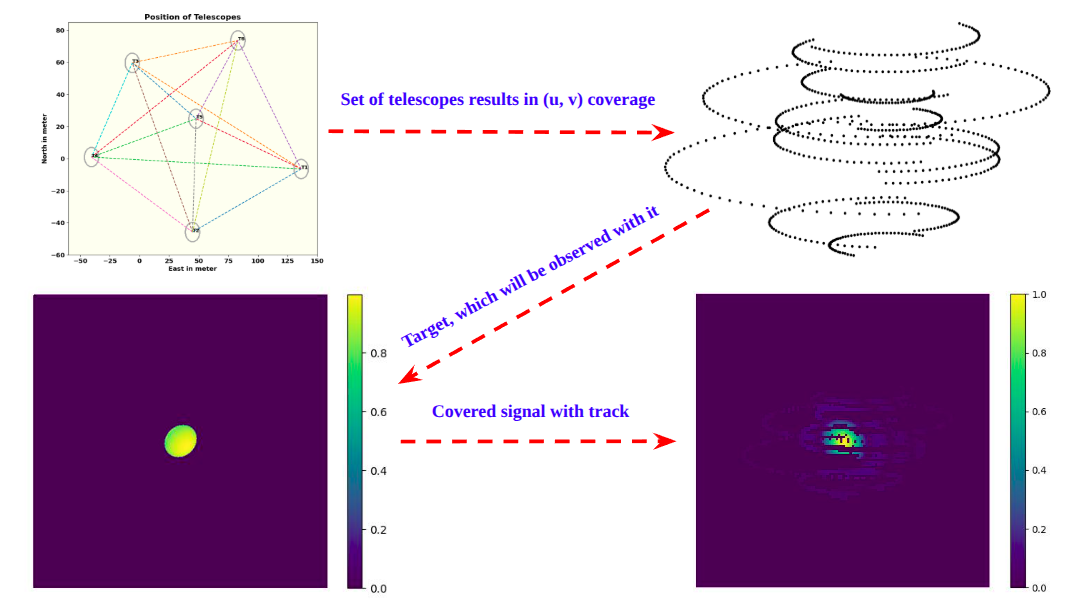
\includegraphics[width=\textwidth]{fig/set.png}
    	\end{figure}
    \end{frame}
    
    \begin{frame}{The Input for GAN}
    	\begin{figure}
    		
\includegraphics[width=0.8\textwidth]{fig/ellipse18.jpg}
    	\end{figure}
    	\begin{itemize}
    		\item Two images are loaded together as input for cGAN
    		\item Sky image as ground truth and observed signal as condition.
    	\end{itemize}
    \end{frame}

    \begin{frame}{The Role of GAN}
    	\begin{columns}[c]
    		\column{0.45\textwidth}
    		\begin{itemize}
    			\item It involves two competing deep neural network models: Generator and Discriminator
    			\item It engage in a zero sum "Minimax" game.
    			\item Pix2Pix cGAN architecture is used here.
    			\item The network is implemented using the TensorFlow library. 
    		\end{itemize}
    		\column{0.55\textwidth}
    	    \begin{figure}
    	    	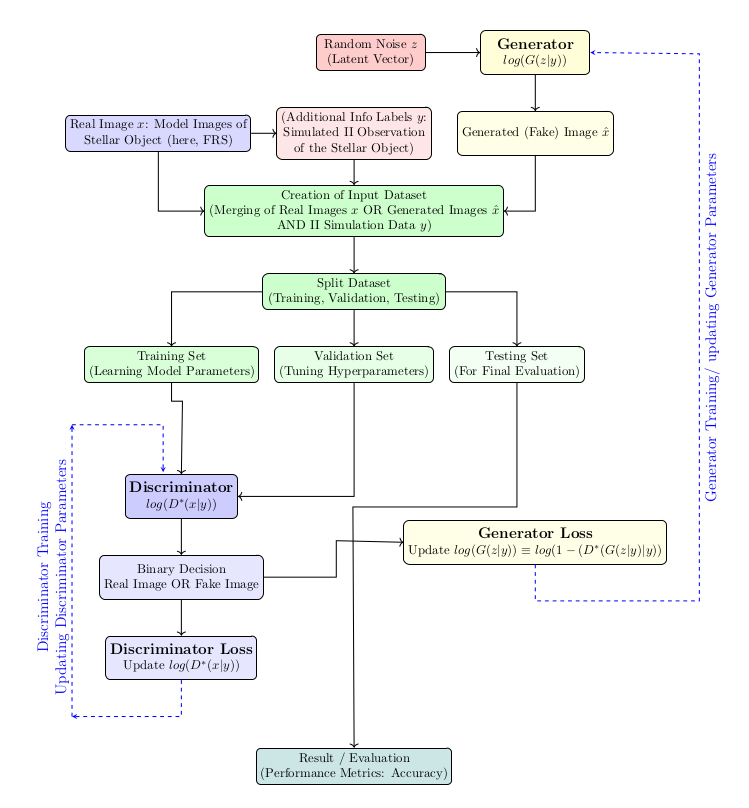
\includegraphics[width=\textwidth]{fig/FlowDiagram_TikZ.png}
    	    \end{figure}
    	\end{columns}
    \end{frame}
    
    \begin{frame}{The Parameters for cGAN}
    	\begin{columns}[c]
    		\column{0.5\textwidth}
    		\begin{itemize}
    			\item The parameters for cGAN are taken based on loss performance of network.
    			 \begin{table}[ht]
    			 	\centering
    			 	\begin{tabular}{ll}
    			 		\hline
    			 		\textbf{Parameter} & \textbf{Value} \\
    			 		\hline
    			 		Learning rate           & 2e-4 \\
    			 		Kernel size             & 5 \\
    			 		Alpha/Beta              & 1 \\
    			 		Batch size              & 1 \\
    			 		Buffer Size             & 1400 \\
    			 		Discriminator repetition  & 1 \\
    			 		Number of Telescope        & 4 \\
    			 		Output Channels         & 1 \\
    			 		Lambda                  & 100 \\
    			 		\hline
    			 	\end{tabular}
    			 \end{table}
    		\end{itemize}
    		
    		\column{0.5\textwidth}
    		\begin{figure}
    			\vspace{-0.7cm}
    			
\includegraphics[width=0.65\textwidth]{fig/Discrep_Runs_Losses_disc_loss.png}
    			
\includegraphics[width=0.65\textwidth]{fig/Discrep_Runs_Losses_gen_total_loss.png}
    		\end{figure}
    	\end{columns}
    \end{frame}

    \begin{frame}{Image Reconstruction: The Result}
    	\begin{figure}
    		\centering
    		
\includegraphics[width=0.9\textwidth]{fig/image_2.png}\hfil
    		
\includegraphics[width=0.9\textwidth]{fig/image_4.png}\hfil
    		
\includegraphics[width=0.9\textwidth]{fig/image_5.png}\hfil
    	\end{figure}
    \end{frame}

    \begin{frame}{Statistical Evolution}
    	\begin{itemize}
    		\item Moments is used for statistical evolution of reconstructed image.
    		\item The raw moment is defined as
    		\begin{equation*}
    			M_{ij} = \sum_{x} \sum_{y} x^i y^j I(x, y)
    			\label{eqn:Mom-ij}
    		\end{equation*}
    		\item The monopole $M_{00}$ defines the total flux.
    		\item The central moment explain the size and shape of the object
    		\begin{equation*}
    			\mu_{pq} = \frac{1}{M_{00}}\sum_{x} \sum_{y} (x - x_c)^p (y - y_c)^q I(x, y).
    			\label{eqn:Central-Mom}
    		\end{equation*}
    		\item The $\mu_{10}$ and $\mu_{01}$ define the x and y centroid
    	\end{itemize}
    \end{frame}
    
    \begin{frame}{Statistical Evolution}
    	\begin{itemize}
    		\item The second order central moments helps to get orientation and semi-major axis
    		\begin{equation*}
    			\theta = \tfrac{1}{2}\arctan \left(\frac{2\mu_{11}}{\mu_{20} - \mu_{02}}\right).
    			\label{eqn:orn}
    		\end{equation*}
    		\begin{equation*}
    			\begin{aligned}
    				&a = 2\sqrt{mp + \delta} \\
    				&b = 2\sqrt{mp - \delta}
    			\end{aligned}
    			\label{eqn:semi}
    		\end{equation*}
    		where,
    		\begin{equation*}
    			mp = \frac{\mu_{20} + \mu_{02}}{2}
    			\label{eqn:mp}
    		\end{equation*}
    		and
    		\begin{equation*}
    			\delta = \frac{\sqrt{4\mu_{11}^2 + (\mu_{20} - \mu_{02})^2}}{2}.	
    			\label{eqn:delta}
    		\end{equation*}
    		
    	\end{itemize}
    \end{frame}
    
    \begin{frame}{Another set of Telescope}
    	\begin{figure}
    		
\includegraphics[width=0.45\textwidth]{fig/telescope.png}
    		
\includegraphics[width=0.45\textwidth]{fig/baseline.png}
    	\end{figure}
    	\begin{itemize}
    		\item The nine telescope of ASTRI, separated on very long scale.
    	\end{itemize}
    \end{frame}
    
    \begin{frame}{Statistical Evolution}
         \begin{figure}
         	\centering
         	
\includegraphics[width=.34\linewidth]{fig/moments/mom0.png}
         	
\includegraphics[width=.34\linewidth]{fig/moments/mom3.png}\hfill
         	
\includegraphics[width=.34\linewidth]{fig/moments/mom4.png}
         	
\includegraphics[width=.34\linewidth]{fig/moments/mom5.png}\hfill
         \end{figure}
    \end{frame}
    
    \begin{frame}{Statistical Evolution}
    	\centering
    	
\includegraphics[width=.34\linewidth]{fig/moments/mom6.png}
    	
\includegraphics[width=.34\linewidth]{fig/moments/mom7.png}\hfill
    	
\includegraphics[width=.34\linewidth]{fig/moments/mom8.png}
    	
\includegraphics[width=.34\linewidth]{fig/moments/mom9.png}
    \end{frame}
    
    \begin{frame}{Statistical Evolution}
    	\begin{itemize}
    		\item The numerical comparison of scatter of the moments of the reconstructed images
    		\item It shows that (u, v) coverage dominate on number of baseline
    	\end{itemize}
    	\tiny
    	\begin{table}
    		\centering
    		\caption{Scatter metrics of the two predicted sets with reference to the set of ground-truth images.}
    		\label{tab:mom}
    		\begin{tabular}{ccccccccc}
    			\toprule
    			Predicted Set & $\mathrm{S}_\mathrm{c}$ & $\mathrm{S}_{11}$ & $\mathrm{S}_{20}$ & $\mathrm{S}_{02}$ & $\mathrm{S}_{12}$ & $\mathrm{S}_{21} $ & $\mathrm{S}_{30}$ & $\mathrm{S}_{03}$ \\
    			\midrule
    			$\mathrm{N6}$ & 0.0223 & 0.387 & 7.606 & 7.296 & 35.822 & 30.603 & 102.691 & 91.102 \\
    			$\mathrm{N9}$ & 0.0256 & 0.499 & 11.446 & 10.869 & 36.159 & 35.865 & 108.123 & 108.622 \\
    			\bottomrule
    		\end{tabular}
    	\end{table}
    \end{frame}

	\begin{frame}
		\begin{center}
			{\fontsize{40}{50}\selectfont \underline{Thank You!!}}
		\end{center}
	\end{frame}

\end{document}